


\subsection{回归对冲和主成分分析}

【chapter11 到 16， 都选自 Bruce Tuckman 和 Angel Serrat 的 Fixed Income Securities，只不过有些是第三版、有些是第四版。FRM 一级关于债券的内容大部分内容也是来源于《Fixed Income Securities》这本书(FRM一级没改版前，很多内容直接选自这本书，改版后很多知识、风格、逻辑延续改版前)。

这个 chapter 和一级知识联系大一些， 并且这个 chapter 在 25 年在选自第四版， 考纲虽然没变， 但是里面很多表达、例子变了】




\subsubsection{DVO l -neutral hedge . }
1. DV01-neutral hedge

\begin{itemize}
\item 【另外， FRM 一级学习的 duration 对冲， 本质上就是 DV01 对冲。这种是理想化的对冲】
\end{itemize}

\begin{itemize}
\item 原版书例子: This section considers the problem of a market maker or a relative value trader on May 14，2021， who purchases \(\$ {100}\) million face amount of the JNJ 2.450s of 09/01/2060 and hedges the resulting interest rate risk by selling the US Treasury 1.625s of 11/15/2050. Because there is no 40-year Treasury bond outstanding， the \({1.625}\mathrm{\;s}\) of \({11}/{15}/{2050}\) ， with about 30 years to maturity， are selected as the best alternative. 【大致含义， 2021 年 5 月 14 日，交易员买入 \(\$ {100}\) million 面值的 40 年期强生债券 (JNJ bond)， 要对冲利率风险。因无 40 年期国债， 选 30 年期国债(30-year Treasury bond )对冲。】
\end{itemize}

\begin{itemize}
\item 并且已知下表信息， 若用 DV01 对冲， 求对冲数量及方向。
\end{itemize}

\begin{center}
\adjustbox{max width=\textwidth}{
\begin{tabular}{|c|c|c|c|}
\hline
Issuer & Bond & Yield & DV01 \\
\cline{1-4}
JNJ & 2.450s of 09/01/2060 & 2.962 & 0.2124 \\
\cline{1-4}
Treasury & 0.875s of 11/15/2030 & 1.601 & 0.0847 \\
\cline{1-4}
Treasury & 1.375s of 11/15/2040 & 2.246 & 0.1446 \\
\cline{1-4}
Treasury & 1.625s of 11/15/2050 & 2.364 & 0.1910 \\
\cline{1-4}
\hline
\end{tabular}
}
\end{center}

\begin{itemize}
\item 解析:DV01 对冲
\end{itemize}

\[
\text{ \$100 million } \times  {0.2124} + {\mathrm{N}}^{ * }{0.1910} = 0
\]

\[
\rightarrow  \mathrm{N} =  - \$ {111.2}\text{ million }
\]

 即需要卖出\$111.2 million 的 30 年国债来对冲风险。

\begin{itemize}
\item DV01 对冲的缺点:
\end{itemize}

\begin{itemize}
\item Assumes that the yields of the JNJ and Treasury bonds move up or down in parallel 平行 【假设被对冲资产(JNJ bonds)和对冲工具(Treasury bonds)的收益率是平行移动的】→当市场利率发生变化时，它们的收益率变化幅度是完全相同的
\end{itemize}

这两种收益率， 即使在相同的市场条件下， 变化也不一致。

而且时间不同，收益率变化也不同。【原版书给出的例子是 40 年的公司债券， 用 30 年的国债对冲】

 改进方式:Regression analysis(一元回归、多元回归)



\subsubsection{ Single-variable regression Hedge 一元回归对冲 }

2. Single-variable regression Hedge 一元回归对冲

\begin{itemize}
\item Regression analysis based on historical data can be applied to improve DV01-neutral hedge approach.
\end{itemize}

\[
\Delta {y}_{t}^{JNJ} = \alpha  + {\beta \Delta }{y}_{t}^{30} + {\varepsilon }_{t}
\]

\(\Delta {y}_{t}^{N}\) : changes in yields of the JNJ bond(target 债券)

\(\Delta {\mathrm{y}}_{\mathrm{t}}^{\mathrm{R}}\) : changes in yields of the 30-year Treasury bonds(对冲债券)

找出 \(\alpha\) 、 \(\beta\) 。

Hedge coefficient or hedge adjustment factor \(\left( \beta \right)\) : the ratio of the average yield change for hedged portfolio to that for the hedging instrument. 国债收益率变化 1BP， JNJ 债券收益率变化 \(\beta\) 个 BP。

回顾: 一元回归 (FRM 一级数量分析科目)

1. 基本概念

\begin{itemize}
\item Linear regression assumes a linear relationship between an explanatory variable \(\mathrm{X}\) and a dependent variable \(\mathrm{Y}\) so that: \(\mathrm{Y} = \alpha  + \beta \mathrm{X} + \epsilon\)  \(\alpha\) =intercept 截距 \(\beta  =\) slope (regression coefficient) \(\varepsilon  =\) shock/innovation/error 2. Ordinary Least Squares
\end{itemize}

\begin{center}
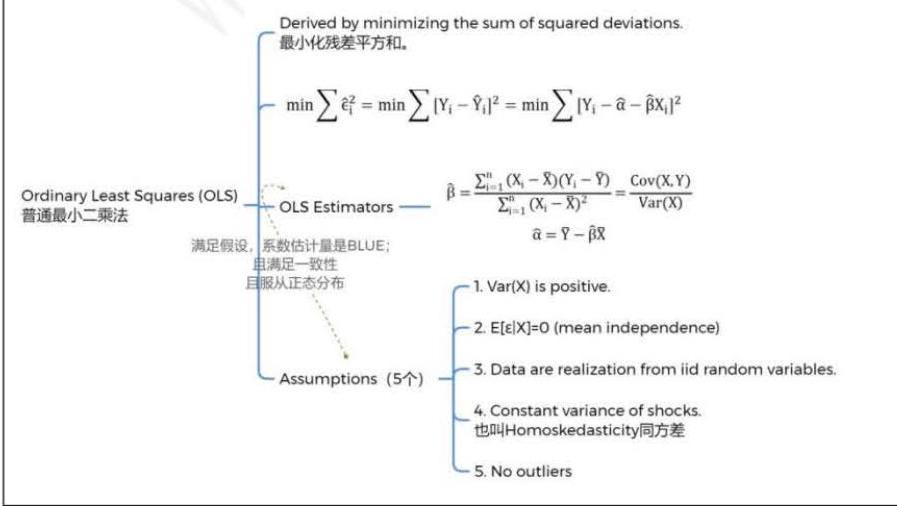
\includegraphics[width=0.7\textwidth]{images/01963dfb-ec81-7114-affc-d6d56ed48aa5_34_361_1448_897_506_0.jpg}
\end{center}
\hspace*{3em} 

\begin{itemize}
\item 继续上面例子。通过回归得出下面信息【怎么回归不要求掌握， 但是要会解读】:
\end{itemize}

\begin{center}
\adjustbox{max width=\textwidth}{
\begin{tabular}{|c|c|c|}
\hline
No. of Observations & 82 & \phantom{X} \\
\cline{1-3}
R-Squared & 77.5\% & \phantom{X} \\
\cline{1-3}
Standard Error & 2.00 & \phantom{X} \\
\cline{1-3}
Regression Coefficients & Value & Std. Error \\
\cline{1-3}
Constant ( \(\widehat{\alpha }\) ) & 0.060 & 0.223 \\
\cline{1-3}
Chg 30yr Treasury Yield \(\left( \widehat{\beta }\right)\) & 0.842 & 0.051 \\
\cline{1-3}
\hline
\end{tabular}
}
\end{center}

\(\beta  = {0.842}\) : the change in the yield of the JNJ bond is only 0.842 times the change in the yield of the Treasury bond， which is very different from a parallel shift.【解读:平均而言， JNJ 债券收益率的变化仅为国债收益率变化的 0.842 倍，这与 parallel shift 平行移动差异很大。在 parallel shift 下， \(\beta  = 1\) . 

回归对冲:

\[
{\mathrm{F}}^{\mathrm{{JNJ}}} \times  \frac{{\mathrm{{DV01}}}^{\mathrm{{JNJ}}}}{100} \times  \beta  + {\mathrm{F}}^{30} \times  \frac{{\mathrm{{DV01}}}^{\mathrm{{JNJ}}}}{100} = 0
\]

【粗糙理解: \({\mathrm{F}}_{\text{ hedge }} =  - {\mathrm{F}}_{\text{ target }} \times  \frac{{\mathrm{{DV01}}}_{\text{ target }}}{{\mathrm{{DV01}}}_{\text{ hedge }}} \times  \beta\) 】

\[
{10}\mathrm{\;{mm}} \times  \frac{0.2124}{100} \times  {0.842} + {\mathrm{F}}^{30} \times  \frac{0.191}{100} = 0
\]

\(\rightarrow  {\mathrm{F}}^{30} =  - {93.6}\mathrm{\;{mm}}\)

即卖出\$93.6 million。

【JNJ bond 收益率对市场利率变动敏感度低，按 DV01 需卖\$111.2 million 国债，因它变动小， 回归对冲考虑此差异， 卖 \$93.6 million 即可对冲利率风险.】

回归对冲优点:

回归对冲使用实际历史数据估计目标债券与对冲债券收益率变化的回归系数，从而更好地捕捉非平行收益率变化(nonparallel shift)的影响。

相较于 DV01 对冲， 回归对冲能更准确地调整对冲比例， 从而更好精准管理、避免过度套期保值的成本与风险



\subsubsection{ Two-Variable Regression Hedge 两元回归对冲 }

3. Two-Variable Regression Hedge 两元回归对冲

【在多元回归中， 主要考虑两元回归， 即两个自变量】

\begin{itemize}
\item Two-variable regression hedges account for the fact that changes in a bond's yield might be better explained by changes in the yields of two other bonds， rather than just one， as in a one-variable regression.
\end{itemize}

4 原版书例子:

 一个交易员认为 20 年期美国国债收益率相对 10 年期和 30 年期过高 (即价格过低)，但直接买入 20 年期国债风险大。

 这个交易员决定使用蝶式策略 butterfly: buy 20-year bonds and sell both 10- and 30- year bonds:

both shorts defend against general rate increases;

the 10-year short defends against flattening; and the 30-year short defends against steepening.

\begin{center}
\adjustbox{max width=\textwidth}{
\begin{tabular}{|c|c|c|}
\hline
No. of Observations & 82 & \phantom{X} \\
\cline{1-3}
R-Squared & 94.7\% & \phantom{X} \\
\cline{1-3}
Standard Error & 1.15 & \phantom{X} \\
\cline{1-3}
Regression Coefficients & Value & Std. Error \\
\cline{1-3}
Constant \(\left( \widehat{\alpha }\right)\) & 0.019 & 0.129 \\
\cline{1-3}
Chg 10yr Treasury Yield \(\left( {\widehat{\beta }}^{30}\right)\) & 0.465 & 0.068 \\
\cline{1-3}
Chg 30yr Treasury Yield \(\left( {\widehat{\beta }}^{10}\right)\) & 0.669 & 0.067 \\
\cline{1-3}
\hline
\end{tabular}
}
\end{center}

\begin{center}
\adjustbox{max width=\textwidth}{
\begin{tabular}{|c|c|c|c|}
\hline
Issuer & Bond 10年期 & Yield & DV01 \\
\cline{1-4}
JNJ & 2.450s of 09/01/2060 & 2.962 & 0.2124 \\
\cline{1-4}
Treasury & 0.875s of 11/15/2030 & 1.601 & 0.0847 \\
\cline{1-4}
Treasury & \phantom{X} & 2.246 & 0.1446 \\
\cline{1-4}
Treasury， & 1.625s of 11/15/2050 & 2.364 & 0.1910 \\
\cline{1-4}
\hline
\end{tabular}
}
\end{center}

问题是这个交易员若有\$100 million face amount of the 20-year bond， 需要卖出多少 10 年期和 30 年期国债?

 解析:

\[
\Delta {y}_{t}^{20} = \alpha  + {\beta }^{10}\Delta {y}_{t}^{10} + {\beta }^{30}\Delta {y}_{t}^{30} + {\varepsilon }_{t}
\]

\({\mathrm{F}}_{\text{ hedge1 }} =  - {\mathrm{F}}_{\text{ target }} \times  \frac{{\mathrm{{DV01}}}_{\text{ target }}}{{\mathrm{{DV01}}}_{\text{ hedge1 }}} \times  {\beta 1} \rightarrow  {\mathrm{F}}_{10} =  - {100} \times  \frac{0.1446}{0.0847} \times  {0.465} =  - \$ {79.44}\)

\({\mathrm{F}}_{\text{ hedge2 }} =  - {\mathrm{F}}_{\text{ target }} \times  \frac{{\mathrm{{DV01}}}_{\text{ target }}}{{\mathrm{{DV01}}}_{\text{ hedge2 }}} \times  {\beta 2} \rightarrow  {\mathrm{F}}_{10} =  - {100} \times  \frac{0.1446}{0.191} \times  {0.669} =  - \$ {50.69}\)

即交易员需要出售\$79.44million 面值的 10 年期国债和\$50.69 million 面值的 30 年期国债。

\begin{itemize}
\item 其他回归形式: 实际做回归时， 也会有其他形式
\end{itemize}

 Level regressions(yields on yields): \({y}_{t} = \alpha  + \beta {x}_{t} + {\varepsilon }_{t}\)

更适合长期趋势分析

\(\diamond\) change regressions(changes in yields on changes in yields): \(\Delta {\mathrm{y}}_{\mathrm{t}} =\)  \({\beta \Delta }{x}_{t} + \Delta {\varepsilon }_{t}\)

在短期对冲中表现更佳


\subsubsection{ Reverse regression 逆回归}

4. Reverse regression 逆回归

\begin{itemize}
\item 在回归(前面的回归)和逆回归(Reverse Regression)中，自变量和因变量通常是互相调换的 \(\rightarrow\) 导致不同的回归系数
\end{itemize}

\begin{itemize}
\item 实际中， 由于变量间的影响并非完全对称， 例如 JNJ bond 收益率对国债收益率的反应和国债收益率对 JNJ 债券收益率的反应可能不同，所以两种对冲方式会有差异
\end{itemize}


\subsubsection{主成分分析 Principal Components Analysis， PCA}


\begin{itemize}
\item 是一种强大的统计工具
\end{itemize}

\begin{itemize}
\item 前面的回归分析用另一些债券的收益率或其变化来解释另外一个债券收益率或其变化。主成分分析， 是对利率进行拆解(从自身出发)， 找出影响利率的要素。要素有很多， PCA 可能只列举其中的一部分因素 Principal Components(PC)。
\end{itemize}

\begin{itemize}
\item 原则:
\end{itemize}

1. The sum of the variances of the PCs equals the sum of the variances of the individual rates. In this sense the PCs capture the volatility of this set of interest rates. 【各个成分的方差之和等于单个利率的方差之和。】

\begin{itemize}
\item 2. The PCs are uncorrelated with each other. While changes in the individual rates are， of course， highly correlated with each other， the PCs are constructed so that they are uncorrelated. 【主成分之间不相关。】
\end{itemize}

3. Subject to these two properties or constraints， each PC is chosen to have the maximum possible variance given all earlier PCs. In other words， the first PC explains the largest fraction of the sum of the variances of the rates; the second PC explains the next largest fraction， etc. 【第一个 PC 最重要，其次是第二 PC】

\begin{itemize}
\item PCA 的优势:
\end{itemize}

通过减少数据的维度，简化了利率变化的描述。

能够捕捉到利率变化中最重要的来源。

提供了一种更简单、更易管理的方法。


拓展:有的书籍通过 PCA 方法， 把影响收益率变化的 PC， 拆分为以下几个:

\hspace*{3em} Level PC 水平移动:

\hspace*{1em} The level movement refers to an upward or downward shift in the yield curve. 【指收益率曲线

\hspace*{3em} 的平行移动 parallel shift】

\hspace*{3em} 在实践中， 水平移动因子解释了收益率总变动的大部分。

\hspace*{2em} Slope PC: 也叫 steepness movement

\hspace*{3em} 非平行移动 non-parallel shift， slope 变， 比如短期利率比长期利率上升更多， 收益率曲线变得

\hspace*{3em} 更陡峭

\hspace*{3em} the shape of the curve

\hspace*{1em} \(>\) Short-rate PC: 也叫 Curvature movement

\hspace*{1em} The curvature movement is a reference to movement in three segments of the yield curve: The

\hspace*{3em} short-term and long-term segments rise while the middle-term segment falls， or vice versa. 【非

\hspace*{3em} 平行移动 non-parallel shift， curvature 变， 比如短期利率和长期利率上升， 而中期利率下降，



\begin{center}
\adjustbox{max width=\textwidth}{
\begin{tabular}{|c|}
\hline
收益率曲线变弯 twist】 其影响是三个因子中最小的。 \\
\cline{1-1}
\hline
\end{tabular}
}
\end{center}








